\chapter{Chance-Constraint Optimization with Kernel Approximation} \label{Technical Approach}

In this chapter, an approach is outlined that allows us to effectively reformulate the chance-constraint problem defined in Section \ref{Problem Statement} using the samples generated using the method described in Chapter \ref{Technical Background}. In Section \ref{SubSec:MMD}, a method to construct a maximum mean discrepancy (MMD) ambiguity sets with kernel approximation is proposed, and in Section \ref{Constraint Reformulation}, the ambiguity set is used to reformulate the chance constraints from Section \ref{Problem Statement}. Finally, in Section \ref{Problem Formulation}, the results are used to define a new OCP.

\section{MMD ambiguity sets} \label{SubSec:MMD}

As the underlying distribution of the data in the constraints \eqref{constraints} is unknown, we first expand them to their distributionally robust counterpart in order to allow for the use of scenarios as an approximation of the distribution. For this, we consider $\tilde{P}$ as the worst case distribution within a set $\mathcal{P}$ of plausible distributions, the so-called ambiguity set. This gives us the new constraints

\begin{equation} \label{wc constraints}
\inf\limits_{\tilde{P} \in \mathcal{P}}\tilde{P} \left[ \text{max}(\boldsymbol{h}(\boldsymbol{u}_{0:H},  \boldsymbol{x}_{0:H},  \boldsymbol{y}_{0:H})) \leq 0 \right] \geq 1 - \alpha.
\end{equation}

To construct the set $\mathcal{P}$, a similarity measure is needed to provide a concrete comparison between various distributions $\tilde{P}$. The Wasserstein metric, a common distance function between probability distributions, has been tried for this purpose in the past. However, most of these works, such as \cite{Hota_19}, limit the class of constraints to affine functions. As such, this approach is not suitable for our general non-linear constraints. In constrast, maximum mean discrepancy \cite{Arthur_12} is able to be applied to non-linear and non-convex constraints. It does that by using the norm of the difference between the kernel mean embeddings (KME) $|| \mu_Q - \mu_{Q'} ||^2_{\mathcal{H}}$ of two distributions $Q$ and $Q'$ as a metric between two distributions. The KME are given as $\mu_Q = \int k(x, \cdot) \text{d}x$ with $k(x, \cdot) \in \mathcal{H}$ being the feature map of the kernel function $k$. The metric can then be rewritten as 

\begin{equation} \label{MMD Kernel}
\text{MMD}(Q, Q') = \text{E}_{z,z' \sim Q}[k(z,z')] + \text{E}_{z,z' \sim Q'}[k(z,z')] - 2\text{E}_{z\sim Q, z' \sim Q'}[k(z,z')]
\end{equation}

The MMD-based ambiguity set $\mathcal{P}$ is then constructed as the set of distributions $\tilde{P}$ in an $\varepsilon$ radius centered around the empirical distribution $P_N$ which is given through the scenarios $\boldsymbol{\delta}^{[1:N]}$. This gives us the set

\begin{equation} \label{ambiguity set}
\mathcal{P} =  \left\{ P : \text{MMD} (P, P_N) \leq \varepsilon \right\}.
\end{equation}

with the empirical distribution being defined as

\begin{equation} \label{empirical distribution}
P_N = \frac{1}{N}\sum_{n = 1}^N d_{\boldsymbol{\delta}^{[n]}}
\end{equation}

with $d_{\boldsymbol{\delta}}$ being a dirac impulse at the point of the sample $\boldsymbol{\delta}$



\begin{figure}[t]
\centering
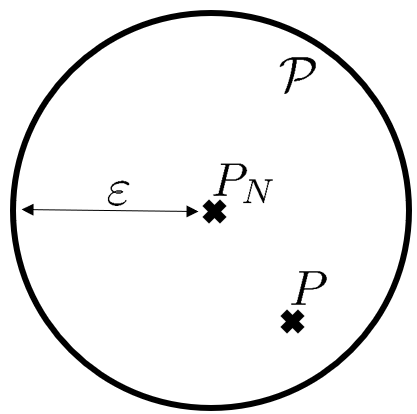
\includegraphics[width= .4\textwidth]{AmbiguitySetDrawing}
\caption{Ambiguity Set $\mathcal{P}$}
\label{AmbiguityPic}
\end{figure}

As illustrated in Figure \ref{AmbiguityPic}, this allows us to build a set near the unknown distribution $P$. As the distribution $P_N$ is built based on the available samples, it represents our best guess at what $P$ looks like. We can assume that for $N \to \infty$, $P_N$ converges towards $P$, but as we only have a limited number of samples available, we also include everything within an $\varepsilon$ radius around $P_N$. We set this radius by constructing a bootstrap MMD ambiguity set as described in \cite{Yassine_22}, which is outlined in Algorithm \ref{alg:Bootstrap}. This procedure requires a number of bootstrap samples $B$ to be chosen and a confidence level $\beta$. It then utilizes kernels $k(\boldsymbol{\delta}^{[i]}, \boldsymbol{\delta}^{[j]}) \in \mathbb{R}$ to define the (biased) MMD estimator as 

\begin{equation} \label{ambiguity set approx}
\widehat{\text{MMD}} (\tilde{P}, P_N) = \sum_{i,j = 1}^N k(\boldsymbol{\delta}^{[i]}, \boldsymbol{\delta}^{[j]}) + k(\tilde{\boldsymbol{\delta}}^{[i]}, \tilde{\boldsymbol{\delta}}^{[j]}) - 2 k(\boldsymbol{\delta}^{[i]}, \tilde{\boldsymbol{\delta}}^{[j]})
\end{equation}

with $\tilde{\boldsymbol{\delta}}^{[n]}, n = 1,...,N$, denoting a bootstrap sample of $P_N$ where samples are drawn with replacement from $\boldsymbol{\delta}^{[1:N]}$. This is done to give us an idea what the empirical distribution might look like with a different set of samples. This can give us insight into how precise our estimate $P_N$ is and what kind of radius $\varepsilon$ should be included in the ambiguity set. We do this by calculating $\widehat{\text{MMD}} (\tilde{P}, P_N)$ for all $B$ bootstrap samples. The results are saved in a list and $\varepsilon$ is chosen as the $\textit{ceil}(B \beta)$-th element of the sorted list. This means we construct the ambiguity set so that $B \beta$ of our bootstrap samples are included while the rest are either outside or on the edge of the ambiguity set.


\begin{algorithm}[t]
	\caption{Bootstrap MMD ambiguity set}
	\label{alg:Bootstrap}
	\hspace*{\algorithmicindent} \textbf{Input}: Scenarios $ \boldsymbol{\delta}^{[1:N]} $, Number of bootstrap samples $B$, Confidence level $\beta$ \\
	\hspace*{\algorithmicindent} \textbf{Output}: Gram matrix $\boldsymbol{K}$, Radius of MMD ambiguity set $\varepsilon$
	\begin{algorithmic}[1]
		\State $\boldsymbol{K} \gets \textit{kernel}(\boldsymbol{\delta}, \boldsymbol{\delta})$
		\For{$m = 1, \dots , B$}
			\State $I \gets N$ numbers from $\{1, \dots N \}$ with replacement
			\State $K_x \gets \sum_{i,j = 1}^N K_{ij};$
			\State $K_y \gets \sum_{i,j \in I} K_{ij};$
			\State $K_{xy} \gets \sum_{j \in I} \sum_{i = 1}^N K_{ij}$;
			\State MMD$[m] \gets \frac{1}{N^2} \left( K_x + K_y - 2 K_{xy} \right) ;$
		\EndFor
		\State MMD $\gets$ \textit{sort}(MMD)
		\State $\varepsilon \gets$ MMD$\left[ \textit{ceil} (B \beta) \right]$
	\end{algorithmic}
\end{algorithm}

\section{Constraint Reformulation} \label{Constraint Reformulation}

With a given MMD ambiguity set $\mathcal{P}$, the feasible set of the constraint \eqref{risk constraints} is given as

\begin{equation} \label{feasible set}
	Z :=  \left\{ \boldsymbol{u}_{0:H} \in \mathcal{U}^{H+1} : \inf\limits_{P \in \mathcal{P}}P \left[ \tilde{h}(\boldsymbol{u}_{0:H},  \boldsymbol{\delta}) \leq 0 \right] \geq 1 - \alpha \right\}.
\end{equation}

with $\tilde{h}(\boldsymbol{u}_{0:H},  \boldsymbol{\delta}) =  \text{max}(\boldsymbol{h}(\boldsymbol{u}_{0:H},  \boldsymbol{x}_{0:H},  \boldsymbol{y}_{0:H}))$.

We can now use the ambiguity set $\mathcal{P}$ defined in section \ref{SubSec:MMD} with the radius $\varepsilon$ to reformulate the feasible set. We are able to reformulate this set using the strong duality proven in \cite{Zhu_20} to get the feasible region

\begin{subequations} \label{feasible region}
  \begin{empheq}[right = \empheqrbrace, left= Z \coloneqq \empheqlbrace \boldsymbol{u}_{0:H} \in \mathcal{U}^{H+1} :]{align}
    & g_0 + \frac{1}{N}\sum_{n = 1}^N g(\boldsymbol{\delta}^{[n]}) + \varepsilon ||g||_\mathcal{H} \leq \alpha \\
    & 1 (\tilde{h}(\boldsymbol{u}_{0:H},  \boldsymbol{\delta}^{[n]})  > 0) \leq g_0 + g(\boldsymbol{\delta}^{[n]}), \; n = 1,...,N \\
    & g_0 \in \mathbb{R}, g \in \mathcal{H}
  \end{empheq}
\end{subequations}

with reproducing kernel hilbert space function $g \in \mathcal{H}$ and $1(\cdot)$ denoting the indicator function. Using this set feasible region exactly is generally intractable in practice. As such, we further approximate the set based on conditional Value-at-Risk (CVaR). For this, we first define the Value-at-Risk (VaR), which is given as 

\begin{equation} \label{VaR definition}
	\text{VaR}_{1-\alpha}^{P} :=  \inf \left\{ t' \in \mathbb{R} : P \left[ \tilde{h}(\boldsymbol{u}_{0:H},  \boldsymbol{\delta}) \leq t' \right] \geq 1 - \alpha \right\}.
\end{equation}

It can be easily shown that

\begin{equation} \label{VaR t0}
	\text{VaR}_{1-\alpha}^{P} \leq 0 \iff  P \left[ \tilde{h}(\boldsymbol{u}_{0:H},  \boldsymbol{\delta}) \leq 0 \right] \geq 1 - \alpha.
\end{equation}

With this, we have an alternative expression of the chance constraints in terms of the VaR. While the VaR constraint is generally nonconvex, we can use the tightest conservative convex approximation given by the conditional convex approximation, which has been shown in \cite{Arkadi_07} to be given by CVaR which is defined as 


\begin{equation} \label{CVaR definition}
	\text{CVaR}_{1-\alpha}^{P} :=  \inf\limits_{t \in \mathbb{R}} \text{E}_P \left[  [\tilde{h}(\boldsymbol{u}_{0:H},  \boldsymbol{\delta}) + t']_+ - t'  \alpha \right]
\end{equation}

with $[\cdot]_+ = \text{max}(0, \cdot)$ denoting the max operator. The constraints can then be expressed as 

\begin{equation} \label{CVaR constr}
\text{CVaR}_{1-\alpha}^{P} \leq 0.
\end{equation}

However, as this constraint depends on the unknown distribution $P$, we use the ambiguity set defined in Section \ref{SubSec:MMD} to relax it. As such, our constraint can be rewritten as 

\begin{subequations}
  \begin{empheq}{align}
	\sup\limits_{\tilde{P} \in \mathcal{P}} \text{CVaR}_{1-\alpha}^{\tilde{P}} &= \sup\limits_{\tilde{P} \in \mathcal{P}}  \inf\limits_{t \in \mathbb{R}} \text{E}_{\tilde{P}} \left[  [\tilde{h}(\boldsymbol{u}_{0:H},  \boldsymbol{\delta}) + t']_+ - t'  \alpha \right] \\
    &= \inf\limits_{t \in \mathbb{R}} \sup\limits_{\tilde{P} \in \mathcal{P}} \text{E}_{\tilde{P}} \left[  [\tilde{h}(\boldsymbol{u}_{0:H},  \boldsymbol{\delta}) + t']_+ - t'  \alpha \right] \leq 0.
  \end{empheq}
\end{subequations}

Applying this to the feasible region defined in \eqref{feasible region}, we arrive at the approximation of the feasible region, which is given as

\begin{subequations}
  \begin{empheq}[right = \empheqrbrace, left= \hat{Z} \coloneqq \empheqlbrace \boldsymbol{u}_{0:H} \in \mathcal{U}^{H+1} :]{align}
    & g_0 + \frac{1}{N}\sum_{n = 1}^N (\boldsymbol{K}\boldsymbol{\gamma})_n + \varepsilon \sqrt{\boldsymbol{\gamma}^\text{T}\boldsymbol{K}\boldsymbol{\gamma}} \leq t' \alpha \label{feasible region Constr1} \\
    & [\tilde{h}(\boldsymbol{u}_{0:H},  \boldsymbol{\delta}^{[n]}) + t']_+ \leq g_0 + (\boldsymbol{K}\boldsymbol{\gamma})_n, \; n = 1,...,N \\
    & g_0 \in \mathbb{R}, \boldsymbol{\gamma} \in \mathbb{R}^N, t' \in \mathbb{R}
  \end{empheq}
\end{subequations}


with $g$ being expressed as the product of the kernel Gram matrix $\boldsymbol{K}$ with the elements $\left[ \boldsymbol{K} \right]_{i, j} = k(\boldsymbol{\delta}^{[i]}, \boldsymbol{\delta}^{[j]})$ and a finite dimensional vector $\boldsymbol{\gamma} \in \mathcal{R}^N$. 

\section{Kernel Approximation} \label{Kernel Approximation}

In Section \ref{Constraint Reformulation}, the chance constraints have been reformulated kernel maximum mean discrepancy where kernels have been used as a universal function approximator based on the available samples. However, for this approximation to be reliable, appropriate kernels must be chosen to give a good estimate. Our samples also consist of multiple elements, i.e., the initial state $\boldsymbol{x}_0$ and the model parameter $\boldsymbol{\theta}$, which are of varying size and magnitude. As such, it is necessary to divide the kernels into multiple factors that are tuned separately and then multiplied.

For these seperate kernels, we use Gaussian kernels $k(z,z') = \text{exp}\left(\text{-}\frac{1}{2\sigma^2} ||z - z'||_2^2 \right)$ with the bandwidth $\sigma$. As such, the elements of the Gram matrix $\boldsymbol{K} \in \mathbb{R}^{N \times N}$ are defined as

\begin{equation} \label{Kernel equation}
K_{ij} = k_{\sigma_\mathcal{X}}(\boldsymbol{x}_0^{[i]}, \boldsymbol{x}_0^{[j]}) k_{\sigma_{\boldsymbol{\Theta}}}(\boldsymbol{\theta}^{[i]}, \boldsymbol{\theta}^{[j]})
\end{equation}

with the kernel for the model parameter $\boldsymbol{\theta}$ being potentially subdivided again into an individual kernel for the process and measurement noise and a kernel for the unknown transition and measurement functions. The individual elements of $\boldsymbol{\sigma} = [\sigma_\mathcal{X}, \boldsymbol{\sigma}_{\boldsymbol{\Theta}}]$ are initialized via the median heuristic \cite{Damien_18} and then increased or decreased to maximize the average probability of a set of $N_\text{test}$ test samples, i.e. find the $\boldsymbol{\sigma}$ that maximizes

 \begin{equation} \label{Average Probability}
\max\limits_{\boldsymbol{\sigma}} \frac{1}{N_\text{test}}  \sum_{n= 1}^{N_\text{test}} \text{P}_{\boldsymbol{\sigma}} ( \boldsymbol{\delta_\text{test}}^{[n]} )
\end{equation}

with the probability function being the product of multiple Gaussian probability functions 

 \begin{equation} \label{Gaussian Probability}
\text{P}_{\boldsymbol{\sigma}} ( \boldsymbol{\delta_\text{test}}^{[n]} ) = \prod_{\sigma_i \in \boldsymbol{\sigma}} \frac{1}{N_\text{train}} \sum_{m = 1}^{N_\text{train}} \frac{1}{\sqrt{2 \pi \sigma_i^2}} k_{\sigma_i}(\boldsymbol{\delta_\text{train}}^{[m]} ,\boldsymbol{\delta_\text{test}}^{[n]})
\end{equation}

over a set of $N_\text{train}$ training samples that are independent of the $N_\text{test}$ test samples.


\section{Problem Formulation} \label{Problem Formulation}

In the previous sections, the chance constraints have been reformulated into a feasible region $\hat{Z}$. We now want to use this to reformulate the chance-constraint OCP defined in section \ref{Problem Statement}. 

For this purpose, we can use the variables $\boldsymbol{\gamma}$, $g_0$ and $t'$ that span the feasible region as optimization parameters while making sure that $\boldsymbol{u}_{0:H}$ is an element of the feasible region.

This way, we can formulate the OCP as

\begin{subequations}
\begin{align}
\begin{split}
\min\limits_{\boldsymbol{u}_{0:H},\boldsymbol{\gamma}, g_0, t' }  J_H(\boldsymbol{u}_{0:H})
\end{split}\\
\begin{split}
\text{s.t.}\; &\forall n = 1,...,N, \;  \forall t = 0,1,...,H
\end{split}\\
\begin{split}\label{systemc1}
&\boldsymbol{x}_{t+1}^{[n]} = \boldsymbol{f}_{\boldsymbol{\theta}^{[n]}} \left( \boldsymbol{x}_{t}^{[n]} , \boldsymbol{u}_t \right) + \boldsymbol{v}_{t}^{[n]}
\end{split}\\
\begin{split}\label{systemc2}
&\boldsymbol{y}_{t} = \boldsymbol{g}_{\boldsymbol{\theta}^{[n]}} \left( \boldsymbol{x}_{t}^{[n]}, \boldsymbol{u}_t \right) + \boldsymbol{w}_{t}^{[n]}
\end{split}\\
\begin{split}\label{systemc3}
 &\boldsymbol{u}_{0:H} \in \hat{Z}(\boldsymbol{\gamma}, g_0, t')
\end{split}
\end{align}
\label{OCP_final}
\end{subequations}

As described in Section \ref{Problem Statement}, we are minimizing a cost function $J_H$. The system dynamics are included through the constraints \eqref{systemc1} and \eqref{systemc2} and must be fulfilled for all scenarios as well. Lastly, the input $u_{0:H}$ is restricted to the feasible set $\hat{Z}$ in \eqref{systemc3} which is defined by the optimization variables $\boldsymbol{\gamma}$, $g_0$ and $t'$.

The optimization problem \eqref{OCP_final} is deterministic and can be solved with well-known methods \cite{Nocedal_06}.




